\documentclass[a4paper,6pt]{article}

% Pacchetti per matematica e circuiti
\usepackage{amsmath, amssymb}
\usepackage{circuitikz}

% Pacchetti per grafica e grafici
\usepackage{graphicx}
\usepackage{pgfplots}
\pgfplotsset{compat=1.17}

% Pacchetti per layout e tabelle
\usepackage{array, multirow, multicol}
\usepackage{geometry}
\geometry{top=2cm, bottom=2cm, left=2cm, right=2cm} % Margini ridotti

% Pacchetti per intestazioni e formattazione accademica
\usepackage{lmodern}
\usepackage{microtype}
\usepackage{fancyhdr}
\pagestyle{fancy}
\fancyhead[C]{\small Prima Esercitazione di Laboratorio} % Intestazione generale centrata
\fancyhead[L,R]{} % Rimuove intestazioni laterali
\fancyfoot[C]{\thepage}

% Pacchetto per i link interattivi senza bordi colorati
\usepackage[hidelinks]{hyperref}

% Impostazioni per il titolo e l’aspetto generale
\title{\Large\textbf{Prima Esercitazione di Laboratorio}\\ \vspace{0.5em} \large Misura di Tensione e Verifica del Teorema di Millman}
\author{\textbf{Gruppo D9:} Saif Edine Safi, Mattia Fait}
\date{\textbf{Ottobre 2024}}

\begin{document}

\maketitle
\tableofcontents % Aggiunge un indice interattivo
\newpage

\section{Introduzione}
L'obiettivo della presente esercitazione è di familiarizzare con gli strumenti tipici del laboratorio di elettronica, come generatori da banco e multimetri. Nella prima parte, studieremo il partitore resistivo, misurando la tensione ai capi di diversi resistori e confrontando i risultati teorici con quelli sperimentali. Nella seconda parte, verificheremo il Teorema di Millman misurando le correnti e le cadute di potenziale nel circuito. Infine, studieremo la caratteristica corrente-tensione (I/V) di un resistore.



\section{Misura di Tensione}


\subsection{Descrizione dell'Esperimento}

\begin{figure}[!ht]
    \centering
    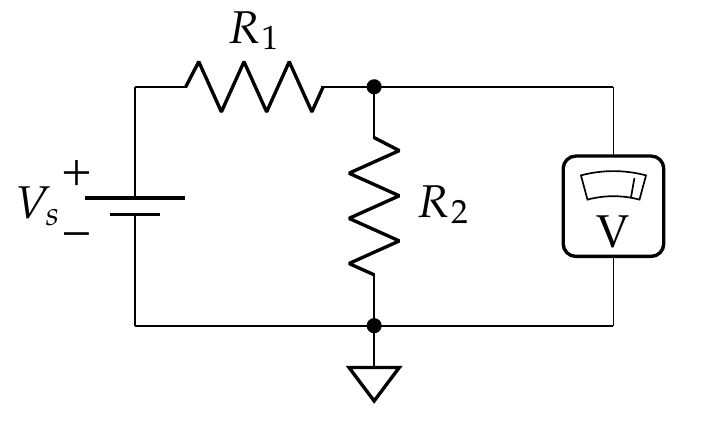
\includegraphics[width=0.3\textwidth]{assets/1.png}
    \caption{Partitore resistivo.}
    \label{fig:primo}
\end{figure}

Il circuito utilizzato consiste in un generatore di tensione \(V_s = 6 V\) collegato in serie a due resistori, \(R_1\) e \(R_2\). Lo scopo è misurare la tensione ai capi del resistore \(R_2\) per diverse coppie di valori di \(R_1\) e \(R_2\). I valori considerati sono:

\begin{itemize}
    \item \(R_1 = 1 k\Omega\), \(R_2 = 1 k\Omega\)
    \item \(R_1 = 1 k\Omega\), \(R_2 = 500 \Omega\)
    \item \(R_1 = 10 k\Omega\), \(R_2 = 10 k\Omega\)
    \item \(R_1 = 100 k\Omega\), \(R_2 = 100 k\Omega\)
    \item \(R_1 = 1 M\Omega\), \(R_2 = 1 M\Omega\)
    \item \(R_1 = 10 M\Omega\), \(R_2 = 10 M\Omega\)
\end{itemize}

Il multimetro da banco è stato utilizzato per verificare che la tensione ai capi di \(R_2\) fosse pari al valore teorico calcolato tramite la legge di Ohm.

\subsection{Dati e Confronto Teorico-Sperimentale}
La tensione ai capi del resistore \(R_2\) è stata calcolata teoricamente utilizzando la formula del partitore di tensione:
\[
V_{R2} = V_s \cdot \frac{R_2}{R_1 + R_2}
\]
I valori misurati e teorici sono riportati nella Tabella \ref{tab:risultati}.

\begin{table}[!ht]
    \centering
    \begin{tabular}{|c|c|c|c|}
        \hline
        \(R_1 [\Omega]\) & \(R_2 [\Omega]\) & \(V_{R2} \text{ (Teorico)} [V]\) & \(V_{R2} \text{ (Misurato)} [V]\) \\
        \hline
        1k & 1k & 3.00 & 2.99 \\
        1k & 500 & 2.00 & 2.00 \\
        10k & 10k & 3.00 & 2.99 \\
        100k & 100k & 3.00 & 2.97 \\
        1M & 1M & 3.00 & 2.85 \\
        10M & 10M & 3.00 & 1.96 \\
        \hline
    \end{tabular}
    \caption{Valori teorici e sperimentali della tensione ai capi di \(R_2\).}
    \label{tab:risultati}
\end{table}

Dai dati ottenuti, si osserva che per valori elevati di resistenza (ordine dei megaohm), la tensione misurata differisce significativamente da quella teorica. Questo comportamento è dovuto alla resistenza interna del multimetro, che non è infinita e introduce un errore significativo quando \(R_1\) e \(R_2\) sono di valore comparabile alla resistenza interna del multimetro.

\subsection{Stima della Resistenza Interna del Multimetro}
Considerando il caso con \(R_1 = R_2 = 10 M\Omega\), è possibile stimare la resistenza interna del multimetro \(R_m\) utilizzando la relazione del partitore di tensione modificata:
\[
V_{R2} = V_s \cdot \frac{R_2 \parallel R_m}{R_1 + (R_2 \parallel R_m)}
\]
Sostituendo i valori misurati, otteniamo:
\[
R_m \approx 9.42 M\Omega
\]
Questo valore suggerisce che il multimetro introduce una resistenza significativa quando misuriamo tensioni su resistenze dell'ordine dei megaohm, alterando i risultati.


\section{Verifica del Teorema di Millman}


\subsection{Descrizione dell'Esperimento}

\begin{figure}[h!]
    \centering
    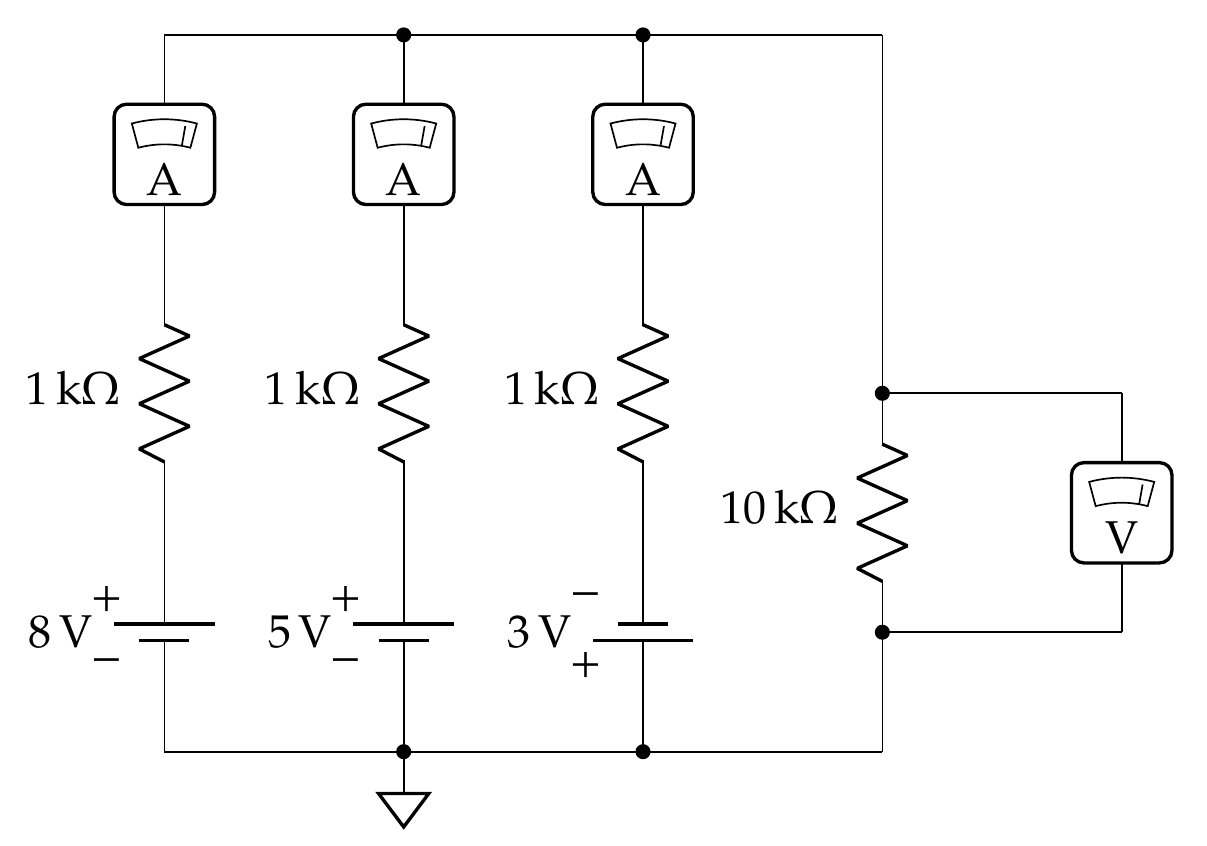
\includegraphics[width=0.3\textwidth]{assets/2.png}
    \caption{Circuito utilizzato per la verifica del Teorema di Millman.}
    \label{fig:millman}
\end{figure}

Il circuito utilizzato per verificare il teorema di Millman è mostrato in Figura \ref{fig:millman}. Esso è composto da tre generatori di tensione e tre resistori in parallelo con un quarto resistore da 10 k\(\Omega\). Lo scopo è misurare le correnti erogate da ciascun generatore e la caduta di potenziale ai capi del resistore da 10 k\(\Omega\).


\subsection{Applicazione del teorema nel circuito sperimentale}

Le misure dei corrispettivi generatori sono:

\begin{table}[h!]
    \centering
    \begin{tabular}{|c|c|c|c|}
        \hline
        \(I_1\) & \(I_2\) & \(I_3\) & \(V_4\) \\ \hline
        4.72 mA   & 1.73 mA    & -6.14 mA  & -3.223 V   \\ \hline
    \end{tabular}
    \caption{Misure sperimentali.}
    \label{tab:esempio}
\end{table}

Utilizzando il teorema di Millman possiamo ricavare il potenziale dell'intero collegamento:

\[
\begin{aligned}
    V_0
    &= \frac{\sum_{i=1}^{4} \left( \frac{V_i}{R_i}\right)}{\sum_{i=1}^{4} \left(\frac{1}{R_i}\right)} \\
    &= \frac{\frac{8V}{1 k \Omega} + \frac{5V}{1 k \Omega} - \frac{- 3V}{1 k \Omega} + \frac{0V}{10 k \Omega}}{\frac{1}{1 k \Omega} + \frac{1}{1 k \Omega} + \frac{1}{1 k \Omega}+ \frac{1}{10 k\Omega}} \\
    & = \frac{100}{31} V \\
    & \approx 3.225 V
\end{aligned}
\]

\[
    V_4 = 0-V_0 =-3.225
\]


Misurando la tensione ai capi del resistore \(R_4\) si vede una differenza di potenziale pari a -3.223 V, dunque il valore sperimentale approssima il valore terico.


\subsection{Stima della corrente di lato}

Attraverso la legge di Ohm e il valore della tensione misurato è possibile stimare la corrente che passa attraverso il resistore: \(I_4 = V_4 / R_4 = -0.32 mA\).

Utilizzando le altre misure è possibile verificare che la stima calcolata sia corretta.
Infatti per la legge di Kirchhoff sui nodi deve risultare che:

\[
I_1 + I_2 + I_3 + I_4 = 0 \Rightarrow 4.72 mA + 1.73 mA -6.14 mA-0.32 mA = -0.01 mA
\]

Il risultato approssima con efficacia lo zero così da confermare la legge di Kirchhoff e dunque validare la corrente stimata sul resistore.

\subsection{Osservazioni}
Applicando il teorema di Millman, il potenziale del nodo comune ai resistori è stato calcolato come:
\[
V_0 = \frac{\sum_{i=1}^{n} \frac{V_i}{R_i}}{\sum_{i=1}^{n} \frac{1}{R_i}}
\]
I valori misurati e teorici hanno mostrato un ottimo accordo, confermando la validità del teorema.



\section{Caratteristica I/V del Resistore}

\subsection{Descrizione dell'esperimento}

\begin{figure}[!ht]
    \centering
    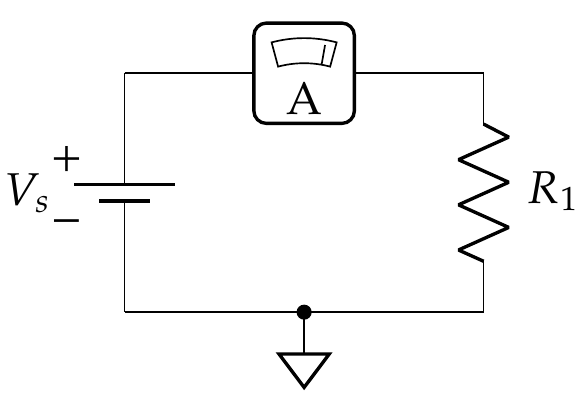
\includegraphics[width=0.3\textwidth]{assets/3.png}
    \caption{Circuito utilizzato per la verifica del Teorema di Millman.}
    \label{fig:Circuito: caratteristica I/V del resistore.}
\end{figure}

Il circuito consiste in un resistore \(R_1\) da 500 \(\Omega\) attaccato ad un generatore di tensione \(V_s\).
L'esperimento consiste nel misurare ripetutamente la corrente che attraversa il resistore, cambiando ogni volta il potenziale ai capi dello stesso.

Le misure hanno lo scopo di verificare sperimentalmente la legge di Ohm.

\subsection{Relazione tra I e V}
 Come si nota dal grafico l'intensità misurata lungo il circutio e la tensione fornita hanno una relazione di tipo lineare,

 Con un modello di regressione lineare è possibile trovare una retta che rappresenti al meglio la relazione fra le due grandezze.

 La retta che si ricava ha equazione \(I=2.02 \frac{mA}{V} V_s -0.14 mA\).

 Il risultato ottenuto coincide con la teoria, infatti la retta teorica calcolata a partire dalla legge di Ohm risulta \(I = \frac{V_s}{R} = 2 \frac{mA}{V} V_s\).

 \begin{table}[!ht]
    \centering
    \begin{tabular}{|c|c|c|}
        \hline
        \(V_s\) [V] & \(I\) [mA] & \(R_1\) [\(\Omega\)] \\ \hline
        0.5 & 0.82 & 609.76 \\ \hline
        1.0 & 1.97 & 507.61 \\ \hline
        1.5 & 2.90 & 517.24 \\ \hline
        2.0 & 3.95 & 506.33 \\ \hline
        2.5 & 4.93 & 507.10 \\ \hline
        3.0 & 5.92 & 506.76 \\ \hline
        3.5 & 6.91 & 506.51 \\ \hline
        4.0 & 7.80 & 512.82 \\ \hline
        4.5 & 8.89 & 506.19 \\ \hline
        5.0 & 9.87 & 506.59 \\ \hline
        5.5 & 10.86 & 506.45 \\ \hline
        6.0 & 11.85 & 506.33 \\ \hline
        6.5 & 13.12 & 495.43 \\ \hline
        7.0 & 14.14 & 495.05 \\ \hline
        7.5 & 15.15 & 495.05 \\ \hline
        8.0 & 16.16 & 495.05 \\ \hline
    \end{tabular}
    \caption{Misure raccolte (senza lampadina)}
    \label{tab:misure_senza_lampadina}
\end{table}






Il circuito per la misura della caratteristica I/V del resistore \(R_1 = 500 \Omega\) ha confermato una relazione lineare tra la corrente e la tensione, in accordo con la legge di Ohm. I dati raccolti sono riportati graficamente nella Figura \ref{fig:regressione_lineare}.

    
\begin{figure}[!ht]
    \centering
    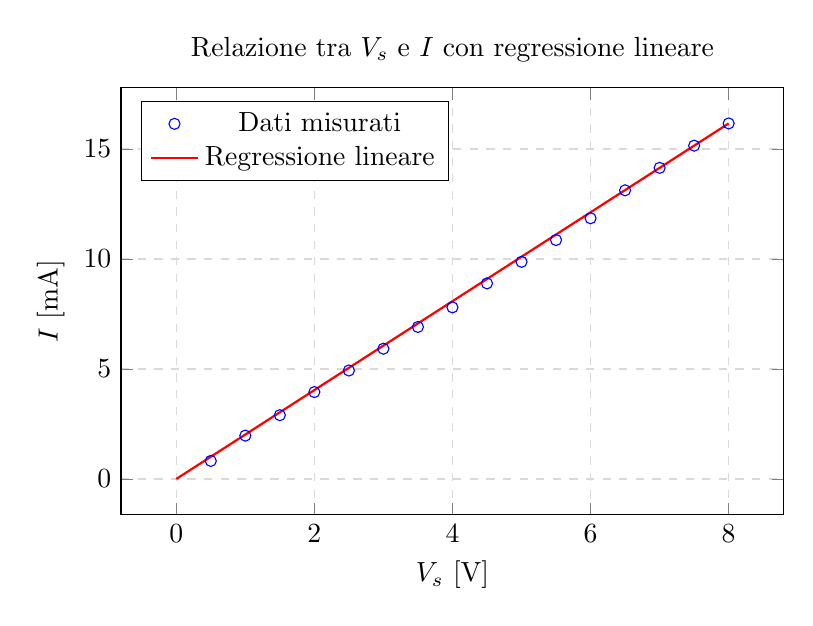
\begin{tikzpicture}
        \begin{axis}[
            xlabel={$V_s$ [V]},
            ylabel={$I$ [mA]},
            title={Relazione tra $V_s$ e $I$ con regressione lineare},
            width=10cm,
            height=7cm,
            grid=major,
            grid style={dashed, gray!30},
            legend pos=north west
        ]
        % Dati misurati
        \addplot[
            only marks,
            mark=o,
            color=blue
        ]
        table[row sep=\\] {
            x       y \\
            0.5     0.82 \\
            1.0     1.97 \\
            1.5     2.90 \\
            2.0     3.95 \\
            2.5     4.93 \\
            3.0     5.92 \\
            3.5     6.91 \\
            4.0     7.80 \\
            4.5     8.89 \\
            5.0     9.87 \\
            5.5     10.86 \\
            6.0     11.85 \\
            6.5     13.12 \\
            7.0     14.14 \\
            7.5     15.15 \\
            8.0     16.16 \\
        };
        \addlegendentry{Dati misurati};

        % Regressione lineare
        \addplot[
            color=red,
            thick,
            domain=0:8
        ]
        {2.02 * x}; % Equazione della retta di regressione
        \addlegendentry{Regressione lineare};
        
        \end{axis}
    \end{tikzpicture}
    \caption{Grafico della corrente \(I\) in funzione della tensione \(V_s\) con retta di regressione lineare}
    \label{fig:regressione_lineare}
\end{figure}


\newpage

\section{Conclusioni}
L'esperimento ha permesso di verificare sia il funzionamento del partitore resistivo sia il Teorema di Millman, evidenziando l'importanza della resistenza interna degli strumenti di misura. Inoltre, la caratteristica I/V del resistore ha confermato la linearità prevista dalla legge di Ohm. La presenza di una resistenza interna non infinita nel multimetro ha introdotto errori significativi nelle misure con resistenze elevate, dimostrando l'importanza di considerare sempre le caratteristiche degli strumenti utilizzati.






\end{document}